
%% bare_conf.tex
%% V1.3
%% 2007/01/11
%% by Michael Shell
%% See:
%% http://www.michaelshell.org/
%% for current contact information.
%%
%% This is a skeleton file demonstrating the use of IEEEtran.cls
%% (requires IEEEtran.cls version 1.7 or later) with an IEEE conference paper.
%%
%% Support sites:
%% http://www.michaelshell.org/tex/ieeetran/
%% http://www.ctan.org/tex-archive/macros/latex/contrib/IEEEtran/
%% and
%% http://www.ieee.org/

%%*************************************************************************
%% Legal Notice:
%% This code is offered as-is without any warranty either expressed or
%% implied; without even the implied warranty of MERCHANTABILITY or
%% FITNESS FOR A PARTICULAR PURPOSE! 
%% User assumes all risk.
%% In no event shall IEEE or any contributor to this code be liable for
%% any damages or losses, including, but not limited to, incidental,
%% consequential, or any other damages, resulting from the use or misuse
%% of any information contained here.
%%
%% All comments are the opinions of their respective authors and are not
%% necessarily endorsed by the IEEE.
%%
%% This work is distributed under the LaTeX Project Public License (LPPL)
%% ( http://www.latex-project.org/ ) version 1.3, and may be freely used,
%% distributed and modified. A copy of the LPPL, version 1.3, is included
%% in the base LaTeX documentation of all distributions of LaTeX released
%% 2003/12/01 or later.
%% Retain all contribution notices and credits.
%% ** Modified files should be clearly indicated as such, including  **
%% ** renaming them and changing author support contact information. **
%%
%% File list of work: IEEEtran.cls, IEEEtran_HOWTO.pdf, bare_adv.tex,
%%                    bare_conf.tex, bare_jrnl.tex, bare_jrnl_compsoc.tex
%%*************************************************************************

% *** Authors should verify (and, if needed, correct) their LaTeX system  ***
% *** with the testflow diagnostic prior to trusting their LaTeX platform ***
% *** with production work. IEEE's font choices can trigger bugs that do  ***
% *** not appear when using other class files.                            ***
% The testflow support page is at:
% http://www.michaelshell.org/tex/testflow/



% Note that the a4paper option is mainly intended so that authors in
% countries using A4 can easily print to A4 and see how their papers will
% look in print - the typesetting of the document will not typically be
% affected with changes in paper size (but the bottom and side margins will).
% Use the testflow package mentioned above to verify correct handling of
% both paper sizes by the user's LaTeX system.
%
% Also note that the "draftcls" or "draftclsnofoot", not "draft", option
% should be used if it is desired that the figures are to be displayed in
% draft mode.
%
\documentclass[conference]{IEEEtran}
% Add the compsoc option for Computer Society conferences.
%
% If IEEEtran.cls has not been installed into the LaTeX system files,
% manually specify the path to it like:
% \documentclass[conference]{../sty/IEEEtran}

%Para garantizar la división correcta de palabras en castellano
\usepackage[spanish,activeacute]{babel}

% idioma
\usepackage[utf8]{inputenc}
\usepackage[spanish]{babel}
\usepackage{pifont}
\usepackage{wasysym}
\usepackage{amssymb}
\usepackage{clrscode}
\usepackage{setspace}
\usepackage{multirow}
\usepackage{verbatim}

\usepackage{listings}

\usepackage{url}

%url
\usepackage{xcolor}
\usepackage[colorlinks=true,urlcolor=blue,linkcolor=blue]{hyperref}
\usepackage{colortbl}
% \usepackage[table]{xcolor}

% Some very useful LaTeX packages include:
% (uncomment the ones you want to load)


% *** MISC UTILITY PACKAGES ***
%
%\usepackage{ifpdf}
% Heiko Oberdiek's ifpdf.sty is very useful if you need conditional
% compilation based on whether the output is pdf or dvi.
% usage:
% \ifpdf
%   % pdf code
% \else
%   % dvi code
% \fi
% The latest version of ifpdf.sty can be obtained from:
% http://www.ctan.org/tex-archive/macros/latex/contrib/oberdiek/
% Also, note that IEEEtran.cls V1.7 and later provides a builtin
% \ifCLASSINFOpdf conditional that works the same way.
% When switching from latex to pdflatex and vice-versa, the compiler may
% have to be run twice to clear warning/error messages.






% *** CITATION PACKAGES ***
%
%\usepackage{cite}
% cite.sty was written by Donald Arseneau
% V1.6 and later of IEEEtran pre-defines the format of the cite.sty package
% \cite{} output to follow that of IEEE. Loading the cite package will
% result in citation numbers being automatically sorted and properly
% "compressed/ranged". e.g., [1], [9], [2], [7], [5], [6] without using
% cite.sty will become [1], [2], [5]--[7], [9] using cite.sty. cite.sty's
% \cite will automatically add leading space, if needed. Use cite.sty's
% noadjust option (cite.sty V3.8 and later) if you want to turn this off.
% cite.sty is already installed on most LaTeX systems. Be sure and use
% version 4.0 (2003-05-27) and later if using hyperref.sty. cite.sty does
% not currently provide for hyperlinked citations.
% The latest version can be obtained at:
% http://www.ctan.org/tex-archive/macros/latex/contrib/cite/
% The documentation is contained in the cite.sty file itself.






% *** GRAPHICS RELATED PACKAGES ***
%


\ifCLASSINFOpdf
\usepackage[pdftex]{graphicx}
%avoid put imagen in specific space
\usepackage{float}
  % declare the path(s) where your graphic files are
  % \graphicspath{{../pdf/}{../jpeg/}}
  \graphicspath{{../images/}}
  % and their extensions so you won't have to specify these with
  % every instance of \includegraphics
\DeclareGraphicsExtensions{.png,.jpeg,}
\else
  % or other class option (dvipsone, dvipdf, if not using dvips). graphicx
  % will default to the driver specified in the system graphics.cfg if no
  % driver is specified.
  % \usepackage[dvips]{graphicx}
  % declare the path(s) where your graphic files are
  % \graphicspath{{../eps/}}
  % and their extensions so you won't have to specify these with
  % every instance of \includegraphics
  % \DeclareGraphicsExtensions{.eps}
\fi
% graphicx was written by David Carlisle and Sebastian Rahtz. It is
% required if you want graphics, photos, etc. graphicx.sty is already
% installed on most LaTeX systems. The latest version and documentation can
% be obtained at: 
% http://www.ctan.org/tex-archive/macros/latex/required/graphics/
% Another good source of documentation is "Using Imported Graphics in
% LaTeX2e" by Keith Reckdahl which can be found as epslatex.ps or
% epslatex.pdf at: http://www.ctan.org/tex-archive/info/
%
% latex, and pdflatex in dvi mode, support graphics in encapsulated
% postscript (.eps) format. pdflatex in pdf mode supports graphics
% in .pdf, .jpeg, .png and .mps (metapost) formats. Users should ensure
% that all non-photo figures use a vector format (.eps, .pdf, .mps) and
% not a bitmapped formats (.jpeg, .png). IEEE frowns on bitmapped formats
% which can result in "jaggedy"/blurry rendering of lines and letters as
% well as large increases in file sizes.
%
% You can find documentation about the pdfTeX application at:
% http://www.tug.org/applications/pdftex





% *** MATH PACKAGES ***
%
%\usepackage[cmex10]{amsmath}
% A popular package from the American Mathematical Society that provides
% many useful and powerful commands for dealing with mathematics. If using
% it, be sure to load this package with the cmex10 option to ensure that
% only type 1 fonts will utilized at all point sizes. Without this option,
% it is possible that some math symbols, particularly those within
% footnotes, will be rendered in bitmap form which will result in a
% document that can not be IEEE Xplore compliant!
%
% Also, note that the amsmath package sets \interdisplaylinepenalty to 10000
% thus preventing page breaks from occurring within multiline equations. Use:
%\interdisplaylinepenalty=2500
% after loading amsmath to restore such page breaks as IEEEtran.cls normally
% does. amsmath.sty is already installed on most LaTeX systems. The latest
% version and documentation can be obtained at:
% http://www.ctan.org/tex-archive/macros/latex/required/amslatex/math/





% *** SPECIALIZED LIST PACKAGES ***
%
%\usepackage{algorithmic}
% algorithmic.sty was written by Peter Williams and Rogerio Brito.
% This package provides an algorithmic environment fo describing algorithms.
% You can use the algorithmic environment in-text or within a figure
% environment to provide for a floating algorithm. Do NOT use the algorithm
% floating environment provided by algorithm.sty (by the same authors) or
% algorithm2e.sty (by Christophe Fiorio) as IEEE does not use dedicated
% algorithm float types and packages that provide these will not provide
% correct IEEE style captions. The latest version and documentation of
% algorithmic.sty can be obtained at:
% http://www.ctan.org/tex-archive/macros/latex/contrib/algorithms/
% There is also a support site at:
% http://algorithms.berlios.de/index.html
% Also of interest may be the (relatively newer and more customizable)
% algorithmicx.sty package by Szasz Janos:
% http://www.ctan.org/tex-archive/macros/latex/contrib/algorithmicx/




% *** ALIGNMENT PACKAGES ***
%
%\usepackage{array}
% Frank Mittelbach's and David Carlisle's array.sty patches and improves
% the standard LaTeX2e array and tabular environments to provide better
% appearance and additional user controls. As the default LaTeX2e table
% generation code is lacking to the point of almost being broken with
% respect to the quality of the end results, all users are strongly
% advised to use an enhanced (at the very least that provided by array.sty)
% set of table tools. array.sty is already installed on most systems. The
% latest version and documentation can be obtained at:
% http://www.ctan.org/tex-archive/macros/latex/required/tools/


%\usepackage{mdwmath}
%\usepackage{mdwtab}
% Also highly recommended is Mark Wooding's extremely powerful MDW tools,
% especially mdwmath.sty and mdwtab.sty which are used to format equations
% and tables, respectively. The MDWtools set is already installed on most
% LaTeX systems. The lastest version and documentation is available at:
% http://www.ctan.org/tex-archive/macros/latex/contrib/mdwtools/


% IEEEtran contains the IEEEeqnarray family of commands that can be used to
% generate multiline equations as well as matrices, tables, etc., of high
% quality.


%\usepackage{eqparbox}
% Also of notable interest is Scott Pakin's eqparbox package for creating
% (automatically sized) equal width boxes - aka "natural width parboxes".
% Available at:
% http://www.ctan.org/tex-archive/macros/latex/contrib/eqparbox/





% *** SUBFIGURE PACKAGES ***
%\usepackage[tight,footnotesize]{subfigure}
% subfigure.sty was written by Steven Douglas Cochran. This package makes it
% easy to put subfigures in your figures. e.g., "Figure 1a and 1b". For IEEE
% work, it is a good idea to load it with the tight package option to reduce
% the amount of white space around the subfigures. subfigure.sty is already
% installed on most LaTeX systems. The latest version and documentation can
% be obtained at:
% http://www.ctan.org/tex-archive/obsolete/macros/latex/contrib/subfigure/
% subfigure.sty has been superceeded by subfig.sty.



\usepackage[caption=true]{caption}
%\usepackage[font=footnotesize]{subfig}
% subfig.sty, also written by Steven Douglas Cochran, is the modern
% replacement for subfigure.sty. However, subfig.sty requires and
% automatically loads Axel Sommerfeldt's caption.sty which will override
% IEEEtran.cls handling of captions and this will result in nonIEEE style
% figure/table captions. To prevent this problem, be sure and preload
% caption.sty with its "caption=false" package option. This is will preserve
% IEEEtran.cls handing of captions. Version 1.3 (2005/06/28) and later 
% (recommended due to many improvements over 1.2) of subfig.sty supports
% the caption=false option directly:
%\usepackage[caption=false,font=footnotesize]{subfig}
%
% The latest version and documentation can be obtained at:
% http://www.ctan.org/tex-archive/macros/latex/contrib/subfig/
% The latest version and documentation of caption.sty can be obtained at:
% http://www.ctan.org/tex-archive/macros/latex/contrib/caption/




% *** FLOAT PACKAGES ***
%
%\usepackage{fixltx2e}
% fixltx2e, the successor to the earlier fix2col.sty, was written by
% Frank Mittelbach and David Carlisle. This package corrects a few problems
% in the LaTeX2e kernel, the most notable of which is that in current
% LaTeX2e releases, the ordering of single and double column floats is not
% guaranteed to be preserved. Thus, an unpatched LaTeX2e can allow a
% single column figure to be placed prior to an earlier double column
% figure. The latest version and documentation can be found at:
% http://www.ctan.org/tex-archive/macros/latex/base/



%\usepackage{stfloats}
% stfloats.sty was written by Sigitas Tolusis. This package gives LaTeX2e
% the ability to do double column floats at the bottom of the page as well
% as the top. (e.g., "\begin{figure*}[!b]" is not normally possible in
% LaTeX2e). It also provides a command:
%\fnbelowfloat
% to enable the placement of footnotes below bottom floats (the standard
% LaTeX2e kernel puts them above bottom floats). This is an invasive package
% which rewrites many portions of the LaTeX2e float routines. It may not work
% with other packages that modify the LaTeX2e float routines. The latest
% version and documentation can be obtained at:
% http://www.ctan.org/tex-archive/macros/latex/contrib/sttools/
% Documentation is contained in the stfloats.sty comments as well as in the
% presfull.pdf file. Do not use the stfloats baselinefloat ability as IEEE
% does not allow \baselineskip to stretch. Authors submitting work to the
% IEEE should note that IEEE rarely uses double column equations and
% that authors should try to avoid such use. Do not be tempted to use the
% cuted.sty or midfloat.sty packages (also by Sigitas Tolusis) as IEEE does
% not format its papers in such ways.





% *** PDF, URL AND HYPERLINK PACKAGES ***
%
%\usepackage{url}
% url.sty was written by Donald Arseneau. It provides better support for
% handling and breaking URLs. url.sty is already installed on most LaTeX
% systems. The latest version can be obtained at:
% http://www.ctan.org/tex-archive/macros/latex/contrib/misc/
% Read the url.sty source comments for usage information. Basically,
% \url{my_url_here}.





% *** Do not adjust lengths that control margins, column widths, etc. ***
% *** Do not use packages that alter fonts (such as pslatex).         ***
% There should be no need to do such things with IEEEtran.cls V1.6 and later.
% (Unless specifically asked to do so by the journal or conference you plan
% to submit to, of course. )


% correct bad hyphenation here$
\hyphenation{
}

\begin{document}

\title{
ANÁLISIS DE FLUJOS DE INFORMACIÓN EN APLICACIONES ANDROID
}

% author names and affiliations
% use a multiple column layout for up to three different
% affiliations
\author{\IEEEauthorblockN{Lina Marcela Jiménez Becerra}
\IEEEauthorblockA{
	Grupo COMIT\\
	Departamento de Ingeniería de Sistemas y Computación\\
	Universidad de Los Andes\\
	Bogotá, Colombia \\
	lm.jimenez12@uniandes.edu.co}
}

% conference papers do not typically use \thanks and this command
% is locked out in conference mode. If really needed, such as for
% the acknowledgment of grants, issue a \IEEEoverridecommandlockouts
% after \documentclass

% for over three affiliations, or if they all won't fit within the width
% of the page, use this alternative format:
% 
%\author{\IEEEauthorblockN{Michael Shell\IEEEauthorrefmark{1},
%Homer Simpson\IEEEauthorrefmark{2},
%James Kirk\IEEEauthorrefmark{3}, 
%Montgomery Scott\IEEEauthorrefmark{3} and
%Eldon Tyrell\IEEEauthorrefmark{4}}
%\IEEEauthorblockA{\IEEEauthorrefmark{1}School of Electrical and Computer Engineering\\
%Georgia Institute of Technology,
%Atlanta, Georgia 30332--0250\\ Email: see http://www.michaelshell.org/contact.html}
%\IEEEauthorblockA{\IEEEauthorrefmark{2}Twentieth Century Fox, Springfield, USA\\
%Email: homer@thesimpsons.com}
%\IEEEauthorblockA{\IEEEauthorrefmark{3}Starfleet Academy, San Francisco, California 96678-2391\\
%Telephone: (800) 555--1212, Fax: (888) 555--1212}
%\IEEEauthorblockA{\IEEEauthorrefmark{4}Tyrell Inc., 123 Replicant Street, Los Angeles, California 90210--4321}}




% use for special paper notices
%\IEEEspecialpapernotice{(Invited Paper)}


%Cambiar el nombre Cuadro por tabla
\renewcommand{\tablename}{Tabla}

% make the title area
\maketitle


\begin{abstract}
%\boldmath
% contexto 
% problema
% propuesta
% evaluacion


\end{abstract}
Controlar el acceso y uso de la información, representa una de las
principales preocupaciones de seguridad en Aplicativos Android.
Un estudio reciente de seguridad en dispositivos móviles, publicado por
McAfee\cite{McAfeeReport}, revela que en el contexto de aplicativos Android:
80\% reúnen información de la ubicación, 82\% hacen seguimiento de alguna acción
en el dispositivo, 57\% registran la forma de uso del celular(mediante Wi-Fi o
mediante la red de telefonía), y 36\% conocen información de las cuentas de
usuario.
Adicionalmente, el informe señala que una aplicación invasiva no necesariamente
contiene malware, y que su finalidad no siempre implica fraude; de las
aplicaciones que más vulneran la privacidad del usuario, 35\% contienen
malware.\\
Si bien, aplicaciones invasivas no necesariamente implican malware y/o acciones
delictivas, el cuestionamiento de fondo es la forma y finalidad con que una
aplicación manipula la información del usuario, y qué garantías puede ofrecer el
desarrollador para que tal manipulación sea consentida.\newline
Partiendo de lo anterior, el presente trabajo de investigación plantea aplicar
técnicas de análisis basadas en control de flujo de información, con el fin de
garantizar el cumplimiento de políticas de seguridad en aplicaciones Android,
desde su construcción.
% For peer review papers, you can put extra information on the cover
% page as needed:
% \ifCLASSOPTIONpeerreview
% \begin{center} \bfseries EDICS Category: 3-BBND \end{center}
% \fi
%
% For peerreview papers, this IEEEtran command inserts a page break and
% creates the second title. It will be ignored for other modes.
\IEEEpeerreviewmaketitle

\section*{Categorías y Descripción de Temáticas}
\label{sec:categorias}
Análisis de flujos de información en aplicaciones.


\section*{Términos Generales}
Técnicas Security-Typed,
Técnicas de flujo de información,
Técnicas de flujo de datos,
Análisis Dinámico,
Análisis estático.




\section*{Palabras Clave}
Jif, 
Políticas de seguridad,
Flujo de información,
Verificación de políticas,
Confidencialidad,
Fuga de información.


\section{Introducción}
En aplicativos Android, el manejo de la información del usuario, es una de las
principales preocupaciones de seguridad. Según un estudio reciente de seguridad
en dispositivos móviles, publicado por McAfee\cite{McAfeeReport}, una importante
cantidad de aplicaciones Android invaden la privacidad del usuario, reuniendo
información detallada de su desplazamiento, acciones en el dispositivo, y su
vida personal.\newline
Por otro lado, para controlar el acceso a información manipulada por sus
aplicaciones, el desarrollador cuenta con los mecanismos de seguridad proveídos
por la API de Android, sin embargo, al estar basados en políticas de control de
acceso, se limitan a verificar el uso de los recursos del sistema acorde a los
privilegios del usuario, lo que suceda con la información una vez sea accedida,
está fuera del alcance de este tipo de controles. Al no contar con herramientas
de análisis de flujo de información en aplicaciones Android, o al utilizar
librerías de terceros, para el desarrollador es difícil verificar
el cumplimiento de políticas de confidencialidad e integridad en la aplicación
próxima a liberar. Por consiguiente, el desarrollador no tiene cómo asegurar la
ausencia de fugas de información en la aplicación.\newline
Si bien, en el campo de aplicativos Android existen diferentes propuestas para
detectar fuga de información, en su mayoría  se enfocan en precisión y
eficiencia del análisis para detectar fugas de datos en aplicaciones de terceros
ya implementadas. Estas propuestas no abordan el problema del lado del
desarrollador, analizando flujos de información de la aplicación para verificar
el cumplimiento de políticas de seguridad.\newline
%  hacen falta propuestas que aborden
% el problema análizando flujo de información, 
% mediante técnicas de lenguajes tipados de seguridad(NO ESTOY SEGURA DE ESTA
% AFIRMACIÓN, ES DECIR QUE SÓLO CON SECURITY-TYPED ES POSIBLE DETECTAR FUGAS
% DE INFORMACIÓN),
% lo que se traduce en
% imposibilidad para detección de fugas mediante sentencias de control, por
% ejemplo, la no detección de flujos implicitos.\newline 
Ante esto, y con el fin de proveer una herramienta de apoyo al desarrollador, de
modo que verifique el cumplimiento de políticas de seguridad en sus
aplicaciones, el presente trabajo aborda el problema de fugas de información en
aplicaciones Android, analizando flujos de información de la aplicación,
mediante técnicas de lenguajes tipados de seguridad.\\
El Articulo está organizado de la siguiente manera: XXX


\section{Contexto}
\subsection{Aplicaciones Android}
En esencia una aplicación Android es una aplicación Java con interfaces
descritas en sintaxis XML, cuya ejecución es activada por el framework la API
Android.\newline 
El framework de Aplicación Android ofrece diferentes funcionalidades de
operación del sistema, proporcionando información de los servicios ofrecidos por
el teléfono. Por ejemplo, provee información de la ubicación del
usuario.\newline 
Así pues, una aplicación Android obtiene del framework, clases e interfaces
necesarias para implementar sus funcionalidades.

Por otro lado, el SDK, Android Software Development Toolkit, permite compilar
la aplicación a una versión ejecutable por dispositivos Android, esto es, código
Dalvik bytecode(.dex). Adicionalmente, el SDK genera el APK, Android Application
Package, donde empaqueta todo el código de la aplicación, incluyendo el
bytecode. El APK es un archivo con extensión .apk, y es el que finalmente se
instala en el dispositivo para obtener las funcionalidades de la aplicación.

En lo que respecta a su estructura, 
una aplicación Android puede integrarse por uno o más de los siguientes
componentes: Activities, Services, Content Providers y Broadcast Receivers.\\
Las actividades representan acciones a ejecutar por el usuario, permiten que el
usuario se comunique con la aplicación.\\
Los servicios son componentes de aplicación que ejecutan tareas en background.\\
Los proveedores de contenido son componentes que permiten compartir datos entre
diferentes aplicaciones Android.\\
Los componentes Broadcast Receivers reciben mensajes enviados por el sistema o
por otras aplicaciones.

Los componentes que integran una aplicación son especificados en el archivo
manifiesto de la aplicación Manifest.xml\cite{App-Manifest}, donde
adicionalmente se declaran: tanto los permisos requeridos por la aplicación para
acceder a partes protegidas de la API\cite{Android-Permissions} e interactuar
con otras aplicaciones; como los permisos requeridos por aplicaciones
externas para interactuar con los componentes de la aplicación.

La comunicación entre varias aplicaciones Android(Comunicación interApp), tiene
lugar a través de intents\cite{App-Intent}, métodos proveídos por la API Android
para la activación de componentes tanto al interior de la aplicación como entre
aplicaciones externas. 

\subsection{Técnicas de análisis de código}
\subsubsection{Análisis estático y dinámico}
Las soluciones propuestas para detectar fuga de información en aplicaciones
Android, se enmarcan en el análisis estático o dinámico de la aplicación, en
algunos casos, se combinan ambos tipos.\newline 
En \textbf{análisis estático}\cite{Static-dynamic}, se estudia el código del
programa para inferir todos los posibles caminos de ejecución. Esto se logra
construyendo modelos de estado del programa, y determinando los estados posibles
a alcanzar por el programa.
No obstante, debido a que existen múltiples posibilidades de ejecución, se opta
por construir un modelo abstracto de los estados del programa. La consecuencia
de tener un modelo aproximado es pérdida de información y posibilidad de menor
precisión en el análisis.\newline 
Por otro lado, en \textbf{análisis dinámico} se ejecuta el programa y se analiza
su comportamiento, verificando el camino de ejecución que ha tomado el programa.
Esa exactitud en la ejecución que se verifica da precisión al análisis, porque
no es necesario construir un modelo aproximado de todos los posibles caminos de
ejecución.

\subsubsection{Técnicas utilizadas en análisis estático} 
Generalmente, para verificar el cumplimiento de políticas de seguridad mediante
análisis estático, se aplican técnicas de seguridad de tipado
(Typed-Inference/Security-Typed Analysis) y técnicas de flujo de
datos(Data/Control Flow Analysis)\cite{Information-Flow-Java}.\newline 
Con \textbf{técnicas Security-Typed} las propiedades de confidencialidad e
integridad son anotadas en el código, y verificadas a tiempo de compilación,
garantizando su cumplimiento a tiempo de ejecución.\newline 
Con \textbf{técnicas de flujo de control} y \textbf{técnicas de flujo de datos},
las políticas de seguridad son verificadas haciendo seguimiento al control de
flujo, o al flujo de datos, respectivamente. Estás técnicas suelen utilizar
grafos de Control de Flujo CFG(Control Flow Graph), Grafos de Flujo de Datos
DFG( Data Flow Graph) y Grafos de llamadas CG (Call Graphs).

\subsubsection{Security Typed Languages}
Las herramientas basadas en técnicas de análisis Security-Typed, involucran
conceptos como flujo de información, políticas de confidencialidad e integridad,
y chequeo de tipos.
\emph{Flujo de información}: el flujo de información describe el
comportamiento de un programa, desde la entrada de los datos hasta la salida de
los mismos.\newline 
\emph{Políticas de confidencialidad e integridad}: confidencialidad e integridad
son políticas de seguridad aplicables mediante control de flujo de información.
Mientras la confidencialidad busca prevenir que la información fluya hacia
destinos no apropiados, la integridad busca prevenir que la información provenga
de fuentes no apropiadas\cite{LanguageIFS-2013}.\newline
\emph{Chequeo de tipos}: al usar un lenguaje tipado de seguridad, las políticas
son definidas a través del lenguaje, porque son expresadas mediante anotaciones
en el código fuente del programa a verificar, y su evaluación se realiza
mediante chequeo de tipos.\newline 
El chequeo de tipos consiste en una técnica estática,
también utilizada para analizar flujo de información durante la compilación de
un programa, más específicamente en la etapa de análisis semántico, el
compilador identifica el tipo para cada expresión del programa y verifica que
corresponda al contexto de la expresión.
Bajo este principio de chequeo, lenguajes tipados de seguridad aplican
políticas de control de flujo, definiendo para cada expresión del programa un
tipo de seguridad(security type), de la forma:  tipo de dato y label de
seguridad(security label). Donde el label de seguridad regula el uso del dato,
acorde a su tipo.\newline 
El compilador realiza el chequeo de tipos, partiendo del conjunto de labels de
seguridad. Así, si el programa pasa el chequeo de tipos y compila correctamente,
se espera que cumpla con las políticas de control de flujo evaluadas.

\subsection{JIF(Java Information Flow)}
% \subsubsection{Sistema de anotaciones en Jif}
Jif es un lenguaje tipado de seguridad que extiende al lenguaje Java con labels
de seguridad, a través de los cuales se especifican restricciones de cómo
debería ser utilizada la información. Jif está compuesto por un compilador y un
sistema de anotaciones.\newline
El análisis de flujo de información de aplicativos Java mediante Jif, requiere
su implementación haciendo uso del sistema de anotaciones de Jif, de modo que se
especifiquen las políticas de seguridad a evaluar.
Tal implementación se basa en adicionar labels de seguridad a la definición
de métodos, variables, arrays, etc; los labels de seguridad no especificados son
generados automáticamente con labels por defecto.\newline
%http://www.cs.cornell.edu/jif/doc/jif-3.3.0/language.html#inference.
La verificación del cumplimiento de las políticas de seguridad, tiene lugar
durante la compilación del aplicativo, allí el compilador Jif aplica chequeo de
labels(label checking)\cite{jifRef},  verificando que los flujos de información
generados cumplen con las restricciones establecidas.

\subsubsection{DML(Decentralized Label Model)}
Jif basa su sistema de anotaciones en el modelo de etiquetas DLM, donde se
manejan tres elementos fundamentales: Principales, Políticas y
Etiquetas.\newline 
Principales: un principal es una entidad con autoridad para observar y cambiar
aspectos del sistema. Un programa pertenece a un principal, quien determina el
comportamiento que este debería tener. Jif cuenta con una serie de principals ya
definidos, por ejemplo, Alice, Bob, Chunck, etc, que pueden ser
utilizados al momento de anotar.\newline 
Políticas: mediante políticas de seguridad el dueño de la política, que es el
principal que la define, determina qué otros principals pueden leer o
influenciar la información. Así, una política puede ser de confidencialidad o de
integridad, y se especifican de la forma: \{owner: reader list\} u
\{owner: writer list\}.\newline 
Etiquetas: una etiqueta consiste en un conjunto de políticas de confidencialidad
e integridad. Las etiquetas se escriben en las expresiones del programa que se
anota(etiquetas de seguridad), esto es métodos, variables, arrays, etc.\newline 
En síntesis, las políticas de seguridad definen que Principales pueden leer o
modificar la información, y esas políticas se expresan mediante
etiquetas.

\subsubsection{Chequeo de etiquetas}
Para hacer seguimiento al flujo de información de un programa, el compilador de
Jif asocia una etiqueta al program counter de cada punto del programa,
etiqueta del progam-counter(\underline{pc}). En cada punto del programa, el
(\underline{pc}) representa la información que podría conocerse tras la
ejecución de ese punto del programa.
El (\underline{pc}) es afectado por las etiquetas con que se define cada
sentencia y expresión del programa, por tanto este es considerado como el límite
superior(máxima información que podría conocerse) de las etiquetas que han
afectado el flujo de información para llegar a un determinado punto de
ejecución.

\subsubsection{Anotación de variables y métodos en Jif}
\label{sssec:sintaxis}
dado que la sintaxis de anotación de Jif se basa en etiquetas de seguridad para
extender la sintaxis del lenguaje java, a continuación se ilustra la forma en
que normalmente se declaran variables y métodos en Java, y la forma en que se
realiza la respectiva extención con la sintaxis de Jif.\newline
\textbf{Definición de variables}\newline
% -Definición de variables: \newline 
En Java la sintaxis para definir una variable es:
\begin{lstlisting}[basicstyle=\scriptsize]
	modifier java-type varName
\end{lstlisting}
Extendiendo la sintaxis Java, en Jif las variables se definen de la forma:
\begin{lstlisting}[basicstyle=\scriptsize]
	modifier java-type {L} varName
\end{lstlisting}
Donde java-type especifica el tipo de dato Java que almacena la variable, \{L\}
la etiqueta de seguridad  para especificar quien es el principal dueño de la
variable, y varName, el respectivo nombre de la variable.\newline
\textbf{Definición de métodos}\newline
en Java la definición de un método tiene la siguiente sintaxis:
\begin{lstlisting}[basicstyle=\scriptsize]
modifier java-type methodName(java-type arg1,,, 
java-type argn){body method}
\end{lstlisting}
En Jif  es posible asociar una etiqueta de seguridad al tipo de dato retornado,
los argumentos que recibe y las excepciones declaradas. 
Adicionalmente, se declara un begin-label(BL) y un end-label(EL).\newline
Cuando en la definición del método no se específica una etiqueta de seguridad,
el compilador de Jif asume unas por defecto. 
La sintaxis es la siguiente:
\begin{lstlisting}[basicstyle=\scriptsize]
modifier java-type{RTL} methodName{BL}(java-type arg1{AL},,,
				java-type argn{AL}) :{EL}
\end{lstlisting}
Donde: \emph{java-type}, es el tipo de dato Java retornado por el
método.\newline 
\emph{RTL}, Return Type Label, indica la etiqueta de seguridad para el valor
retornado por el método.\newline 
\emph{BL}, Begin Label, representa el máximo nivel se seguridad del
\underline{pc} desde donde se invoca el método, de este modo,
la etiqueta del program counter desde donde se invoca el método debe ser
menor o igual de restrictivo que el BL con que se define el método. El BL
también asegura que el método sólo podrá actualizar partes del programa que
tengan igual BL. Con tales restricciones se evita la generación de flujos
implícitos, vía invocación del método.\newline
\emph{AL}, Argument Label, indica el máximo nivel de seguridad para los
argumentos con que se llama el método, así, las etiquetas de los argumentos con
que se invoca el método deben ser menor o igual de restrictivos que el AL con que ha
definido el método.\newline 
\emph{EL}, End Label, indica el \underline{pc} en el punto de terminación del
método, y representa el máximo nivel de información que puede conocerse tras la
finalización del método.

\subsubsection{Labels de anotación que Jif asume por defecto}
\label{sssec:default-labels}
Cuando en la declaración de variables o métodos no se especifica su respectivo
label de seguridad, Jif lo infiere o genera automáticamente. De acuerdo al tipo
de sentencia. Así:\newline
- Variables locales: Jif infiere sus labels, de modo que se respeten las
restricciones sobre el flujo de información.\newline
- Arrays: por defecto, Jif define el label público para el Base Label(BL) y el
Size Label(SL) de un array.\newline
- Class fields: el label por defecto es \{ \}, que representa información con el
menor nivel de confidencialidad. Es el label menos confiable, con este se
asegura que información altamente confidencial no podrá ser almacenado en el
campo de la clase.\newline
- Métodos: los labels que Jif genera por defecto para la definición de
métodos son:\newline 
Argument Label(AL): el label por defecto es el Top principal, es decir que sólo
la máxima autoridad podrá leer la información del argumento.\newline 
Begin Label(BL): su label por defecto es el Top principal.\newline
End Label(EL): Jif hace un Join de los labels con que se definen las
excepciones del método, si el método no tiene excepciones, el label por defecto
es el menos restrictivo \{ \}\newline
Return Type Label(RTL): Jif hace un Join de los AL y el EL.\newline
Labels para excepciones: el valor del EL.

\subsubsection{Flujos implícitos y \underline{pc}}
Los flujos implícitos son canales creados durante el control de flujo del
programa. Buscando prevenir la fuga de información a través de estos canales,
Jif asocia un \underline{pc} a cada statement y expresión del programa,
representando la información que debería conocerse tras su evaluación.\\
El sistema de tipos de Jif asegura que el \underline{pc} debe ser por
lo menos tan restrictivo como los labels de las variables de que depende el
program counter de la sentencia.\newline
En el siguiente ejemplo se ilustra la generación de flujos implícitos:
\begin{lstlisting}[basicstyle=\scriptsize]
boolean {Alice:} secreto;
boolean {} publico;
secreto = true;
if( secreto )		
	publico = 0;
else				//Implicit Flow
	publico = 1;
\end{lstlisting}
El flujo implícito tiene lugar en el condicional porque la variable
\emph{publico}, cuyo nivel de seguridad es bajo (\underline{pc}=\{\}) permite
conocer información de la variable \emph{secreto}, con nivel de seguridad alto
(\underline{pc}=\{Alice:\})\newline

\section{Descripción del Problema}
\label{sec:problema}
En Android, por defecto, el desarrollador no cuenta con mecanismos para
definir políticas de confidencialidad e integridad que regulen
el flujo de información de sus aplicaciones. Siendo complejo prevenir fugas de
información del usuario, puesto que, el desarrollador carece de herramientas que
le garanticen la ausencia de flujos indeseados.\newline
Precisamente, una de las principales preocupaciones de seguridad en aplicativos
Android, es la manipulación de información del usuario.
Así lo evidencia un
estudio reciente de seguridad en dispositivos móviles, publicado por
McAfee\cite{McAfeeReport}, este señala  que una importante cantidad de
aplicaciones Android invaden la privacidad del usuario, reuniendo información
detallada de su desplazamiento, acciones en el dispositivo, y su vida personal.
De este modo, 80\% reúnen información de la ubicación, 82\%
hacen seguimiento de alguna acción en el dispositivo, 57\%
registran la forma de uso del celular(mediante Wi-Fi o
mediante la red de telefonía), y 36\% conocen información de
las cuentas de usuario.\newline
Las motivaciones para este tipo de acciones varían acorde al tipo de
información, por ejemplo: monitorear información de ubicación para mostrar
publicidad no solicitada; seguir las acciones sobre el dispositivo, para conocer
qué aplicaciones son rentables de desarrollar, o para ayudar a aplicaciones
maliciosas a evadir defensas; acceder a información de cuentas del usuario con
fines delictivos; obtener información de contactos y calendario
del usuario, buscando modificar los datos; obtener información del
celular(número, estado, registro de MMS y SMS) para interceptar llamadas y
enviar mensajes sin consentimiento del usuario.\newline 
Con o sin autorización de acceso, existen motivaciones suficientes para que un
tercero desee manipular información del usuario.\newline
Adicionalmente, el informe señala que una aplicación invasiva no necesariamente
contiene malware, y que su finalidad no siempre implica fraude; de las
aplicaciones que más vulneran la privacidad del usuario, 35\% contienen
malware.\newline 
Si bien, aplicaciones invasivas no necesariamente implican malware y/o acciones
delictivas, el cuestionamiento de fondo es la forma y finalidad con que una
aplicación manipula la información del usuario, y qué garantías puede ofrecer el
desarrollador para que tal manipulación sea consentida.

La falta de control sobre los flujos de información de la aplicación puede
ocasionar fugas de información, generando problemas de seguridad tanto para
quien la implementa como para quien la usa.\newline
Como contramedida a este problema, la API de Android ofrece herramientas de
seguridad basadas en políticas de control de acceso, y el desarrollador puede
implementarlas en su aplicación. Sin embargo, estos mecanismos se centran en
regular el acceso de los usuarios del sistema a determinados recursos, y no en
verificar qué sucede con la información una vez es accedida. 

Para superar dicha carencia, diferentes trabajos de investigación han abordado
el problema de fuga de información en aplicaciones Android, tanto desde un enfoque
dinámico como desde un enfoque estático, la literatura existente al
respecto(TaintDroid\cite{TaintDroid}, Flow-Droid\cite{FlowDroid-Thesis},
DidFail\cite{DidFail}, DroidForce\cite{DroidForce}), indica que la mayoría de
propuestas hacen data-flow analysis mediante técnicas de análisis 
tainting, partiendo del bytecode
Enfocándose en la precisión y eficiencia del análisis para detectar fugas de
datos en aplicaciones de terceros ya implementadas. Por consiguiente,
la finalidad del análisis no es garantizar el cumplimiento de políticas de
confidencialidad e integridad desde la construcción del aplicativo.

Partir de tales propuestas para analizar aplicaciones propias y garantizar
políticas de confidencialidad e integridad desde su construcción, puede implicar
incompletitud en el análisis(under-tainting) y no detección de flujos
implícitos. Esto debido a que,
% aún cuando el
% desarrollador conoce la funcionalidad de su propio código, las optimizaciones
% realizadas por el compilador pueden adicionar complejidad al
% mismo\cite[pag.~43]{SecureProgramming}; 
por un lado, al realizar análisis tainting de forma dinámica, el marcado de
datos se propaga únicamente a través de caminos del programa actualmente
ejecutados. Así, si existen datos que son influenciados por los datos marcados,
pero no están dentro de los actuales caminos de ejecución, quedan sin la
propagación de la marca, dando lugar al problema de
undertainting\cite{dynamic-tainting}\cite{Bit-Level-Taint-Analysis}. Es
decir, se obtiene precisión en el análisis, pero se pierde completitud.\newline
Por el otro, aún cuando se hace análisis tainting de forma estática, y el
marcado de datos puede ser propagado para todos los caminos posibles de
ejecución  del programa, superando el inconveniente de under-tainting, la
detección de flujos implícitos es posible si, en la construcción de la
herramienta de análisis se propaga el marcado de datos para flujos
implícitos\cite{taint-analysis}. 
Sin embargo, las propuestas que basan su análisis en data-flow estático,
suelen restringir la propagación del marcado de datos a flujos explícitos,
ganando eficiencia en el análisis. Las propuestas mencionadas anteriormente, no
son ajenas a tal generalidad(DidFail\cite{DidFail}[page 33],
FlowDroid\cite{FlowDroid-Thesis}[page 30]).

Ahora bien, la falta de garantías en el cumplimiento de determinadas
políticas de seguridad en la aplicación que se implementa, puede superarse
usando control de flujo de información, Information Flow Control(IFC), puesto
que, con esta técnica la aplicación  es analizada estáticamente  para
identificar todos los posibles caminos que podrían tomar sus flujos de
información, garantizando que a tiempo de ejecución, la aplicación respeta
determinadas políticas de seguridad.

Finalmente, partiendo del contexto que se plantea, donde es el propio
desarrollador Android quien requiere evaluar políticas de seguridad en su
aplicación, para  garantizarle al usuario que la aplicación las cumple. Resulta
apropiado proveerle una herramienta de apoyo, mediante la cual analice el flujo
de información de la aplicación que implementa, y verifique el cumplimiento
de políticas de seguridad.

\section{Propuesta}
\label{sec:propuesta}
La presente sección inicia con una descripción de alto nivel del diseño de
solución que se propone. Después, describe detalladamente los elementos que
conforman la propuesta de solución: \ref{sub:politica} y
\ref{sub:lineamientos}.\newline

Para garantizarle al usuario que la aplicación que implementa respeta
determinadas políticas de seguridad, el desarrollador Android requiere de una
herramienta que le permita: primero definir las políticas de seguridad a
evaluar, y segundo, verificar el cumplimiento de las políticas
definidas.\newline 
Así pues, la propuesta para cumplir con tales requerimientos consiste en proveer
una herramienta de análisis de flujo de información, mediante en el sistema de
anotaciones del lenguaje tipado de seguridad Jif. Se propone partir de Jif
porque este ofrece un sistema de anotaciones basado en un modelo de
etiquetas(DLM), más un módulo de verificación(compilador de Jif),
tal como se ilustra en la figura \ref{fig:desingReal}.
De este modo, con anotaciones en el código de su aplicación, el desarrollador
puede definir políticas de seguridad, para luego validar con el módulo de
verificación, si la aplicación respeta tales políticas.\newline 
Ahora bien, el principal reto para llevar a cabo dicha propuesta, es permitir el
análisis de flujo de información de aplicativos Android con el sistema de
anotaciones de Jif, puesto que, Jif sólo permite el análisis de flujo de
información en aplicativos Java convencionales, y una de las diferencias entre
una aplicación Android y una aplicación Java convencional es la API de Android,
puesto que, para adquirir sus funcionalidades una aplicación Android requiere de
clases de la API. No obstante, el sistema de anotaciones de Jif está
implementado para clases del lenguaje Java estándar y no para clases de la API
Android.\newline 
En consecuencia, el diseño ideal para contribuir con la solución del problema es:
una herramienta que contenga el setup de Jif para Android, e integre un clasificador de sources
y sinks. De modo que, la herramienta analice flujos de información en
aplicativos Android, verificando que cumplan con las políticas de seguridad que
el desarrollador ha definido.\newline 
El Setup de Jif para Android hace referencia a las clases de la API Android con
anotaciones Jif(Anotaciones a la API), estas anotaciones son necesarias porque
es a través de la API que la aplicación escribe o lee información de los sources
y los sinks, generando flujos de información entre los mismos. Por ende, el
análisis de flujo de información entre sources y sinks con el sistema de
anotaciones de Jif, implica anotaciones a clases de la API. 

Si bien, el diseño ideal requiere anotaciones a toda la API, para efectos del
presente trabajo se limita el Setup de Jif, partiendo de una política de
seguridad específica.
Por consiguiente, el diseño se centra en soportar un conjunto reducido de clases
de la API de Android, y en incluir un conjunto específico de sources y
sinks; de acuerdo a una política de seguridad establecida. Ese conjunto de
sources y sinks, se toma del listado de sources y sinks proveído por
SuSi(\ref{sec:susi}) .\newline
Adicionalmente, para aspectos de evaluación, se incluye el diseño de un anotador
que automatiza la anotación requerida por el desarrollador.
De manera que, acorde a la política de seguridad establecida, se genere la
versión anotada del aplicativo a analizar.\newline
La figura \ref{fig:desingReal} muestra el esquema del diseño, allí los componentes
principales son el \emph{generador de anotaciones} y la \emph{herramienta de
análisis estático}.\newline 
Para retornar la versión Jif del aplicativo, el \emph{generador de anotaciones}
parte del código fuente de la aplicación Android a analizar, la política de
seguridad a evaluar, y los sources y sinks requeridos para verificar tal
política.\newline 
Luego esa versión Jif del aplicativo se debe pasar como entrada a la herramienta
de análisis estático, la cual retorna el análisis de flujo de
información.\newline 
La \emph{herramienta de análisis estático}, está integrada
por el compilador de Jif(Módulo de verificación) y las anotaciones a la API de
Android.

\begin{figure}[t!]
	\begin{center} 
	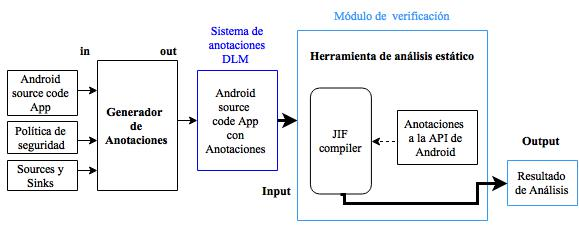
\includegraphics[width=8.8cm]{desing3Real-2-2-colors-2.jpg} 
	\end{center}
	\caption{Diseño herramienta de análisis estático.\newline
	Partiendo del código fuente del aplicativo Android, la política de seguridad a
	evaluar, más los sources y sinks requeridos para verificar la política; el
	generador de anotaciones retorna la versión anotada del aplicativo a analizar.
	Luego la versión anotada del aplicativo se pasa como entrada a la herramienta
	de análisis estático, la cual retorna el resultado de análisis de flujo de información.}
	\label{fig:desingReal}
\end{figure}

Siguiendo el esquema de diseño anteriormente descrito: primero, se define la
política de seguridad a evaluar \ref{sub:politica}; y segundo, se definen los
lineamientos de anotación \ref{sub:lineamientos}.

\subsection{Definición de la política de seguridad}
\label{sub:politica}
Detectar si una aplicación Android presenta flujos de información entre:
información con nivel de seguridad alto e información con nivel de seguridad bajo.\newline
\textit{Información con nivel de seguridad alto}: la información
catalogada con nivel de seguridad alto hace referencia a un conjunto de sources.
Los sources representan información confidencial o privada del usuario, por
tanto, el usuario quisiera tener el control de hacia donde se dirige tal
información.
El conjunto de sources está integrado por los métodos getDeviceId,
getSimSerialNumber, findViewById, getLatitude, getLongitude y getSubscriberId.
Adicional a estos métodos, se incluye el tipo de dato EditText, si y sólo si, el
campo UI al que hace referencia corresponde a un campo tipo textPassword(campos
destinados a almacenar contraseñas).\newline 
\textit{Información con nivel de seguridad bajo}: la
información considerada con nivel de seguridad bajo, comprende un conjunto
de sinks. Los sinks son canales que permiten la salida de información del
dispositivo, por ejemplo, los mensajes de texto. El conjunto de sinks
está integrado por los métodos de la clases Log y SmsManager de la API.

\subsection{Lineamientos de anotación}
\label{sub:lineamientos}
Los lineamientos de anotación definen los elementos básicos de anotación
\ref{subsec:elements}, anotaciones necesarias para la API de Android
\ref{subsec:api} y anotaciones en los aplicativos a analizar \ref{subsec:anotador}.

\subsubsection{Elementos básicos de anotación}
\label{subsec:elements}
Para anotar la información con su respectivo nivel de seguridad alto o bajo, de
modo que, partiendo de tales anotaciones se evalúe la existencia de flujos de
información entre información con nivel de seguridad alto e información con
nivel de seguridad bajo, se define una autoridad para los programas, también se
definen las etiquetas de seguridad para especificar las políticas de seguridad.
Así:\newline 
Principal \emph{Alice}: haciendo uso de los principales ya definidos en Jif, se
establece al principal \emph{Alice} como la autoridad máxima. Este principal
tendrá todo el poder para actuar sobre aspectos de los programas.\newline
Política para anotar información con nivel de seguridad alto: la etiqueta de
seguridad \emph{\{Alice:\}},  indica que la información tiene nivel seguridad
alto, es decir, que se trata de información sensible o privada.\\
Variables con nivel de seguridad alto deben ser anotadas con tal label de
seguridad, porque esté específica que sólo el dueño de la información(Alice)
puede acceder a la misma.\newline 
Política para anotar información con nivel de seguridad bajo: la etiqueta de
seguridad \emph{\{\}}, indica que la información tiene nivel de seguridad bajo,
es decir, información de conocimiento público.\newline


\subsubsection{Anotaciones a la API de Android}
\label{subsec:api}
%\textbf{(b)Anotaciones a la API de Android}\newline

\begin{figure}[t!]
	\begin{center}
	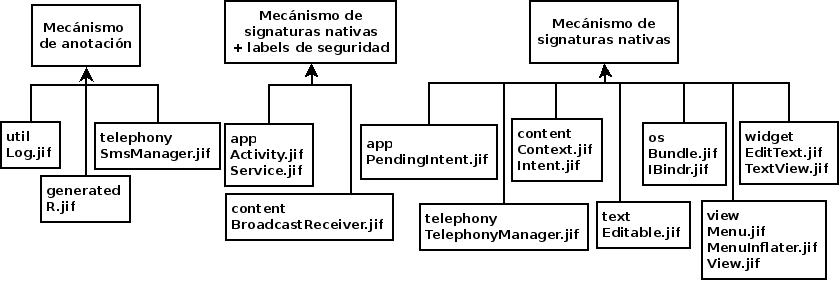
\includegraphics[width=8.5cm]{annotationsMechanims.jpeg}
	\end{center}
	\caption{Mecanismos de anotación para clases de la API.}
	\label{fig:annotationsMechanims}  
\end{figure}
dado que la API de Android provee las librerías necesarias para implementar las
funcionalidades de una aplicación Android, permitiendo a su vez, que el
aplicativo escriba o lea información de los métodos sources y sinks, las clases
pertenecientes a la API generan flujos de información. Así, para verificar la
política de seguridad previamente definida, se requieren anotaciones tanto a las
clases que definen los sources y sinks en que se centra la política, como
anotaciones a clases y librerías requeridas en la implementación de las
aplicaciones, por ejemplo, las clases que permiten implementar componentes
de actividades, servicios y broadcast receivers.\newline 
En el caso de los sinks la anotación tiene un propósito adicional, este es,
controlar el flujo de información que se envía a través de los mismos, la
definición de los métodos de las clases Log y SmsManager de la API Android,
deben anotarse de tal manera que, se controle el nivel de seguridad de los
argumentos con que se invocan tales métodos.\newline 
Para esto se utilizan las etiquetas de seguridad que regulan el llamado a
métodos en el sistema de anotaciones de Jif(sintaxis de anotación
\ref{sssec:sintaxis}), estas son Begin Label(BL) y Argument Label(AL).
Con las etiquetas para el BL se determinan los puntos del programa desde donde
puede ser invocado el método, de este modo, el método podrá ser invocado si: el
nivel de seguridad del punto del programa desde donde se llama el método es
menor o igual de restrictivo que el BL con que ha sido definido el método. Para
el presente caso se busca que un método pueda ser invocado desde cualquier punto
del programa.\newline
Con las etiquetas para los argumentos del método, AL, se controla el nivel de
seguridad de los argumentos con que se invoca el método. Por tanto, el nivel de
seguridad de los argumentos con que se invoca un método, debe ser menor o igual
de restrictivo que el nivel de seguridad con que han sido definidos los
argumentos del método.\newline
El nivel de restricción de la información se evalúa de acuerdo a las
etiquetas de seguridad con que de defina e invoque el método. De este modo,
información con nivel de seguridad alto es más restrictiva que información con nivel de
seguridad bajo.
Aterrizando estos conceptos a los elementos definidos en 
\ref{subsec:elements}, información anotada con el label \emph{\{Alice:\}} es
más restrictiva que información anotada con el label \emph{\{\}}. Puesto que, el
primer label denota que la información tiene nivel de seguridad alto, mientras
que el segundo, indica que la información tiene nivel de seguridad bajo.\newline 
Tomando como ejemplo el método sendTextMessage de la clase SmsManager, mediante
el cual se envían mensajes de texto:
\begin{lstlisting}[basicstyle=\scriptsize]
sendTextMessage(String destinationAddress, String scAddress, 
	String text, PendingIntent sentIntent, 
	PendingIntent deliveryIntent){}
\end{lstlisting}

Se tiene que el parámetro \emph{text} es el que recibe la información a enviar,
y por tanto esa información debe ser pública.\newline 
Por consiguiente, en la definición del método la etiqueta de seguridad del
argumento(AL) correspondiente a la información a enviar(sms), se anota con la
etiqueta pública \{\}.
Con tal etiqueta se garantiza que la información se envía, si y sólo si, el
nivel de seguridad del argumento con que se invoca el método es menor o igual de
restrictivo que la etiqueta pública \{\}; como no se tiene una etiqueta de
seguridad menos restrictiva que esta, se garantiza que la información sólo es
enviada si efectivamente está anotada con tal etiqueta, es decir, si se trata
de información pública.\newline 
Por ejemplo,
si el método se invoca con información anotada con label de seguridad alto, se
genera un flujo de información indebido, dando lugar a un error en la
compilación del programa que le llama.\newline 
En el caso del BL al anotarlo con la etiqueta \{Alice:\}, se permite que el
método sea invocado desde cualquier punto de un programa, es decir, desde
puntos con nivel de seguridad bajo(\{\}) y desde puntos con nivel de seguridad
alto(\{Alice:\}).
Para el resto de labels se dejan los que Jif genera por
defecto(\ref{sssec:default-labels}) .\newline
% cualquier punto de un programa que sea igual o menor de restrictivo que el
% principal Alice, esto se traduce en que podrá ser invocado desde cualquier punto
% de un programa, lo cual es correcto porque lo que se busca el evitar que se
% envíe información considerada con nivel se deguridad alto y no, evitar que el
% método sea utilizado. Poner ejemplo XXXX?\newlie
Continuando con el ejemplo del método sendTextMessage y aplicando lo
anteriormente descrito, este método se anota de la siguiente manera:
\begin{lstlisting}[basicstyle=\scriptsize]
sendTextMessage{Alice:}(String{Alice:} destinationAddress, 
	String{Alice:}scAddress, 
	String{} text, 
	PendingIntent{Alice:} sentIntent,
	PendingIntent{Alice:} deliveryIntent) { }
\end{lstlisting}

El principio de anotación propuesto es aplicable para los métodos de la clase
Log, ya que estos también representan sinks.\newline 
Tales criterios de anotación son aplicados a través del mecanismo fundamental de
anotación que provee el sistema de anotaciones de Jif, en el cual se implementa
la respectiva versión Jif de la clase, esto es, anotando con etiquetas de
seguridad las variables, definición y cuerpo de los métodos de la clase.
Adicional a este mecanismo de anotación(mecanismo de
anotación\footnote{Para referenciar los mecanismos utilizados en la integración
de clases de la API Android, al sistema de anotaciones de Jif, se adoptan los
nombres: mecanismo de anotación, mecanismo de signaturas nativas y mecanismo de
signaturas nativas más labels de seguridad.}), el compilador de Jif provee un
mecanismo que permite interactuar con código de clases Java ya
existentes\cite{annotations-Jif}, para esto, se recurre a signaturas nativas.
Así, se implementa una versión Jif de una clase Java ya existente, en la que se
declaran signaturas nativas proveídas por Jif, constructor y métodos necesarios
de la clase(mecanismo de signaturas nativas).
Al mecanismo de signaturas nativas también se puede  adicionar labels de
seguridad(mecanismo de signaturas nativas más labels de seguridad).\newline 
% Para incluir el resto de clases de la API requeridas en la verificación de la
% política de seguridad establecida, por ejemplo, las clases que pertmiten definir
% componentes de aplicación como Activity.java(para la implementación de
% componentes de actividades), se recurre a esos mecanismos adicionales.
La figura \ref{fig:annotationsMechanims} resume las clases a anotar de acuerdo
al mecanismo con que se integran al sistema de anotaciones de Jif.
\subsubsection{Anotaciones en los aplicativos a analizar}
\label{subsec:anotador}
\begin{figure}[t!]
	\begin{center}
	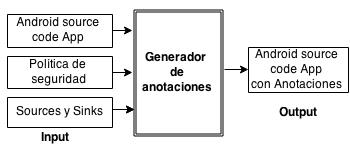
\includegraphics[width=6cm]{desingSolution2-2.jpg}
	\end{center}
	\caption{Entradas y salidas para el generador de anotaciones.\newline
	Para generar la versión anotada del aplicativo a analizar, el anotador parte
	del código fuente del aplicativo, la política de seguridad definida, más el
	conjunto de sources y sinks requeridos para la misma.}
	\label{fig:desingSolution}
\end{figure}
Si bien, el desarrollador debe implementar manualmente las anotaciones en el
aplicativo a analizar, acorde a las políticas de seguridad que requiere
verificar; en el presente diseño de solución, se incluye un generador de
anotaciones que automatiza la anotación requerida por el desarrollador. Como se
ilustra en la figura \ref{fig:desingSolution}, el generador de anotaciones
retorna la versión anotada del aplicativo a analizar, partiendo del código
fuente del aplicativo, la política de seguridad y el conjunto de sources y
sinks, necesarios para verificar la política de seguridad.\newline
La anotación del aplicativo se fundamenta en identificar la declaración de
sources, y en verificar qué métodos influencian esa información, de modo que,
cuando la información sea enviada a través de sinks, tenga el nivel de seguridad
adecuado. Así, las políticas de anotación definidas en \ref{subsec:elements} son
aplicadas a variables y métodos, de acuerdo a si contienen o no información del
conjunto de sources, integrado por: el tipo de dato EditText(cuando el campo UI
al que referencia corresponde a un campo que almacena contraseñas), y los
métodos:
getDeviceId, getSimSerialNumber, findViewById, getLatitude, getLongitude y getSubscriberId.\newline
Finalmente, se define una serie de pasos que permiten aplicar las políticas de
anotación definidas, y esos pasos son automatizados mediante el generador de
anotaciones.













\section{Trabajos Relacionados}
\label{sec:trabajo}
\subsection{Clasificación de Sources y Sinks(SuSi)}
\label{sec:susi}
En el ámbito de análisis de seguridad de aplicaciones, independientemente del
tipo de análisis, estático o dinámico, el punto de partida es la definición de
políticas de seguridad, los pasos sucesivos para detectar la perdida de
información giran en torno a tales políticas.\newline
Muchas de las propuestas para análisis de flujo de información en aplicaciones
Android, parten de un listado de sources y sinks para definir sus políticas de
privacidad. Así, en el grupo de \textbf{sources} se incluyen las fuentes de
datos sensibles, mientras que en el grupo de \textbf{sinks}, se incluyen los
medios o canales que podrían filtrar información sensible de forma no autorizada. 
En consecuencia, la efectividad del análisis se ve limitada al listado de
sources y sinks, y la veracidad de los mismos. El inconveniente con estos sources y sinks, es que su
clasificación suele hacerse de forma manual, por tanto, existe mayor
probabilidad de error u omisión.\newline
Con el fin de precisar dicha clasificación, el trabajo de investigación
\textbf{SuSi} propone el uso de machine-learning para la clasificación y
categorización de sources y sinks, partiendo del código fuente de la API Android.
La propuesta de análisis se materializa en una herramienta que: partiendo del
código fuente de una determinada versión de la API de Android, retorna un
listado con la respectiva categorización de sources y sinks.\newline
El proceso de análisis se compone de dos rondas secuenciales: clasificación y
categorización.\newline
Así, la salida de la primera ronda: calsificación de sources y sinks, se
convierte en entrada para la ronda de categorización, donde se definen
diferentes tipos de categorías, 12 para sources y 15 para sinks.
\subsection{JOANA}
\label{JOANA-Tool}
JOANA (Java Object-sensitive ANAlysis)- Information Flow Control Framework for
Java\cite{JOANA}. Verifica si una aplicación java contiene fugas de
información, mediante análisis estático de flujos de información. El análisis parte  de anotaciones en
el código fuente de la aplicación. JOANA utiliza técnicas de análisis de flujo de
datos y técnicas de análisis de control de flujo. El frontend de la herramienta
está basado en el framework de análisis de programas WALA\cite{wala}, a partir
del cual obtiene la representación intermedia del código Java en forma SSA(Static
Single Assignement), lo que permite obtener información dinámica del programa.
Por otro lado, utiliza Grafos de Dependencia, System Dependence Graphs(SDG),
para detectar dependencias entre las sentencias del programa, es decir,
si existen caminos entre sentencias etiquetadas con nivel de seguridad
alto y sentencias con nivel de seguridad bajo. Para esta etapa del análisis
recurre a técnicas de slicing y chopping, reduciendo la cantidad de caminos
posibles sólo a los válidos. Así obtiene como resultado, una mayor precisión y
reducción de falsas alarmas en el análisis.

Aunque JOANA provee sencillez a la hora de anotar el código a analizar, pues
sólo es necesario anotar inputs y outputs del programa, porque la herramienta se
encarga de propagar las anotaciones en el resto del programa; carece de
características adicionales ofrecidas por sistemas de tipado de seguridad, por
ejemplo, el mecanismo downgrading facilitado por JIF.

Si bien, al igual que JOANA, la herramienta propuesta a través del presente
trabajo, aplica análisis de control de flujo de información, esta última busca
analizar aplicaciones implementadas en código Android, aprovechando las ventajas
del sistema de anotaciones de JIF. Proporcionando una herramienta de apoyo al
desarrollador de aplicaciones Android, ya que por el momento, JOANA sólo analiza
aplicaciones en JAVA.

\subsection{JoDroid}
\label{subsec:jod}
JoDroid\cite{JoDroid-Paper} es una extensión a la herramienta de análisis JOANA
para soportar análisis de aplicaciones Android.\newline 
El análisis de JOANA está basado en Program Dependence Graphs(PDG) y técnicas
slicing. Con PDGs obtiene una representación del programa que
analiza, donde los nodos representan statements y expresiones; y las aristas
modelan las dependencias sintácticas entre los statements y expresiones:
dependencias de datos y dependencias de control, por tanto el grafo está en
capacidad de modelar, tanto flujos explícitos como flujos implícitos.\newline
Con técnicas slicing provee sensibilidad al contexto, puesto que el PDG se
construye de manera tal que al hacer el backwards slice de un determinado nodo,
se obtiene cada nodo que es alcanzable por caminos del grafo que conservan
llamadas al contexto.\newline
El PDG es generado mediante el Front-end de WALA, framework que analiza bytecode
de Java. Así, los ajustes hechos a JOANA adaptan parte del Front-end de WALA
para generar el PDG de aplicaciones Android.\newline
JoDroid detecta tanto flujos explícitos como flujos implícitos.

\subsection{FlowDroid}
\label{FlowDroid-Tool}
FlowDroid es una herramienta para análisis estático de flujo de datos en
Aplicaciones Android. También permite el análisis de aplicaciones Java.\newline
Esta herramienta utiliza un tipo especial de análisis de flujo de datos:
análisis tainting, que hace seguimiento al flujo de datos entre un conjunto de
sources y un conjunto de sinks. Define tales conjuntos a partir de
SuSi[\ref{sec:susi}], un clasificador automático de sources y sinks para la Api
de Android.\newline 
FlowDroid provee un alto recall y precisión\cite{FlowDroid-Thesis} en el
análisis. El recall, mediante un fiel modelamiento del ciclo de vida de una
aplicación Android; la precisión, incluyendo elementos de análisis como:
context-, flow-, field- y object-sensitive. Para proveer sensibilidad al flujo y
al contexto, recurre a grafos de llamada; y con grafos que modelan todos los
procedimientos del programa(inter-procedural control-flow graph), analiza el
flujo de datos entre procedimientos, proporcionando field- y object-sensitive.\newline
Los autores de esta propuesta, alcanzan precisión en la construcción del grafo
de llamadas extendiendo Soot\cite{Soot}, un framework que genera código
intermedio para código Java y código ejecutable Android(dex). Adicionalmente,
con el framework Heros\cite{heros}, incluyen llamadas multihilos en el análisis
de flujo de datos entre procedimientos.

Entre las limitaciones de FlowDroid está el over-tainting y la no detección
de flujos implícitos. Por tanto, la herramienta no distingue elementos marcados
ni dentro de arrays, ni dentro de collections, si se inserta un elemento marcado
dentro de alguna de estas estructuras, inmediatamente se marca el resto de
elementos. La herramienta tampoco identifica flujos implícitos,    
% causados por dependencias entre control de flujo.\newline
puesto que, según los resultados de evaluación de
DroidBench\cite{DroidBenchBenchmarks}, su benchmark; cuando Flowdroid analiza el
conjunto de aplicaciones de prueba para la identificación de flujos implícitos, no
detecta fuga de datos, generando falsos negativos en la detección de flujos
implícitos\cite[pags 32-36]{FlowDroid-Thesis}.

Aún cuando el problema a atacar es el mismo: fuga de información, la propuesta
que se expone a través del presente trabajo difiere en el enfoque de análisis de
FlowDroid, mientras FlowDroid se concentra en detectar si la aplicación de un
tercero presenta fugas de información, la herramienta planteada aborda el
análisis del lado del desarrollador de la aplicación, apoyándolo en
la verificación del cumplimiento de políticas de seguridad. Así, resulta más
conveniente guiar el análisis mediante control de flujo de información, ya que
se previene fuga por datos no marcados para el análisis(under-tainting) y por
la no detección de flujos implícitos, siendo posible garantizar el cumplimiento
de políticas de seguridad.
 
\subsection{TaintDroid, Dinamic Taint Tracking, para la detección de fugas de
Información}
\label{TaintDroid-Tool}
A diferencia de las propuestas expuestas anteriormente, caracterizadas
por ejecutar el análisis de manera estática, TaintDroid es una herramienta de
análisis dinámico. Está herramienta extiende la plataforma de dispositivos
celulares Android, con el fin de verificar el uso dado por aplicaciones de
terceros a datos sensibles del usuario. El análisis aplica técnicas de análisis
tainting, marcando automáticamente como sources, datos provenientes de fuentes
consideradas privadas y/o sensibles; y como sinks, canales para la salida de
datos de la aplicación, como por ejemplo internet.
Cada vez que un dato marcado como source sale de la aplicación, se genera un log.\newline 
Para reducir sobrecarga en el dispositivo, pues el análisis es ejecutado a nivel
de instrucciones, instrumentan la máquina virtual de Android con marcas de
propagación a nivel de: variables, métodos, mensajes y archivos. Las marcas de
variable hacen seguimiento a datos dentro de aplicaciones consideras no
confiables. Las marcas de mensaje siguen mensajes entre aplicaciones. Debido a
que TaintDroid no hace seguimiento a la ejecución de código nativo, utiliza las
marcas de métodos para hacer seguimiento a lo retornado luego de invocar métodos
de librerías nativas. Las marcas de archivo son utilizadas para verificar la
persistencia de los datos, acorde a las políticas de seguridad.\newline
Otra medida para reducir sobrecarga en la ejecución del análisis, consiste en
omitir flujos de control, generando no detección de flujos
implícitos\cite[pag 12]{TaintDroid}.\newline Si bien, TaintDroid supera el inconveniente de sobrecarga en la ejecución del
análisis, un inconveniente característico en análisis dinámico, está limitado
para detectar fuga de datos mediante flujos implícitos, puesto que se
enfoca en hacer seguimiento a flujos de datos directos(flujos
explícitos).

Al ser una herramienta de análisis dinámico, TaintDroid sólo detecta fugas de
información correspondiente a las ejecuciones presentadas por el programa, y
para la finalidad de su análisis: informar al usuario de posibles fugas de
información, se puede decir que es adecuado. No obstante, para los propósitos de
la propuesta planteada a través del presente trabajo, con la que se pretende
brindar una herramienta de análisis para que el desarrollador verifique el
cumplimiento de políticas de seguridad en la aplicación que implementa, no
resulta viable aplicar análisis dinámico, ni técnicas de análisis tainting para
hacer seguimiento a flujos de datos.

\section{evaluación}
\label{sec:eval}
Esta sección inicia presentando el conjunto de evaluación del que se parte para
evaluar la herramienta de solución propuesta(Prototipo), más las métricas de
seguridad a verificar.
Después compara los resultados de analizar el conjunto de evaluación con
el Prototipo, y otras dos herramientas: FlowDroid y JoDroid.

\subsection{Conjunto de evaluación y métricas}
Para la evaluación se parte de DroidBench versión
1.0\cite{DroidBenchBenchmarks}, DroidBench es un benchmark creado
específicamente para evaluar propiedades de seguridad en aplicaciones Android.
De este benchmark se toma un grupo de testcases que permiten evaluar la política
de seguridad establecida(\ref{sub:politica}), tal grupo está integrado por
20 testcases, de los cuales, 14 presentan fugas de información. En la tabla
\ref{tb:conjunto} se listan los casos de prueba.
\begin{table}[t]
\begin{center}
\small
\resizebox{6cm}{!}{
\begin{tabular}{|p{0,5cm}|p{5,2cm}|}
 	\hline
 	\multicolumn{2}{|c|}{\cellcolor{gray!30}Conjunto de Evaluación} \\
	\hline
	\textbf{Test} & \textbf{Nombre Testcase}\\
	\hline
	1 & AndroidSpecific\_DirectLeak1\\
	\hline
	2 & AndroidSpecific\_InactiveActivity\\
	\hline
	3 & AndroidSpecific\_LogNoLeak\\
	\hline
	4 & AndroidSpecific\_Obfuscation1\\
	\hline
	5 & AndroidSpecific\_PrivateDataLeak2\\
	\hline
	6 & ArraysAndLists\_ArrayAccess1\\
	\hline
	7 & ArraysAndLists\_ArrayAccess2\\
	 \hline
	8 & GeneralJava\_Exceptions1\\
	\hline
	9 &  GeneralJava\_Exceptions2\\
	\hline
	10 & GeneralJava\_Exceptions3\\
	\hline
	11 & GeneralJava\_Exceptions4\\
	\hline
	12 & GeneralJava\_Loop1\\
	\hline
	13 & GeneralJava\_Loop2\\
	\hline
	14 & GeneralJava\_UnreachableCode\\
	\hline
	15 & ImplicitFlows\_ImplicitFlow1\\
	\hline
	16 & ImplicitFlows\_ImplicitFlow2\\
	\hline
	17 & ImplicitFlows\_ImplicitFlow4\\
	\hline
	18 & Lifecycle\_ActivityLifecycle3\\
	\hline
	19 & Lifecycle\_BroadcastReceiverLifecycle1\\
	\hline
	20 & Lifecycle\_ServiceLifecycle1\\
	\hline
\end{tabular}
}
\end{center}
\caption{Conjunto de evaluación.
Donde \textit{Test} identifica el caso de prueba y \textit{Testcase} especifica
el nombre de la aplicación de caso de prueba.}
\label{tb:conjunto}
\end{table}
% % \vspace{-0.5em}
Este conjunto de prueba es analizado con FlowDroid, JoDroid y con el Prototipo. 
El Prototipo representa la herramienta de análisis propuesta, por tanto, con el
Prototipo se genera la versión anotada del aplicativo y se evalúa la política
anotada.\newline
Los calificativos para los resultados del análisis son:  
True Positive(TP): cuando se reporta un leak que efectivamente existe. 
False Positive(FP): cuando se reporta un leak que no existe.  
True Negative(TN): cuando no se reporta leak y efectivamente no existe. 
False Negative(FN): cuando no se reporta un leak existente.\newline
Adicionalmente, con el comando \textit{time}\cite{time-man} de unix, se mide el
tiempo(desempeño) que tarda cada herramienta en ejecutar el análisis.\newline
En base a los resultados de análisis que reporta cada herramienta, se
calcula su respectiva Precisión y Recall.\newline
La \textbf{Precisión} hace referencia a los Casos Positivos esperados(correctos
e incorrectos: TP, FP), en contraste con la proporción de verdaderos Positivos(TP)
detectados\cite{Precision-Recall}. Una alta Precisión indica que la herramienta
reporta más correctos Positivos(TP) que incorrectos Positivos(FP).\newline 
El \textbf{Recall} indica la proporción de Casos Positivos detectados(TP),
frente a los Casos Positivos esperados como correctos\cite{Precision-Recall}. Un
alto Recall indica que la herramienta reporta más correctos Positivos(TP) que incorrectos
Negativos(FN), es decir, la herramienta deja pasar menos errores.\newline
Las fórmulas para calcular Precisión(p) y Recall(r), son:
\begin{equation}
\label{pre}
	p = TP/(TP +FP) 
\end{equation}
\begin{equation}
\label{rec}
	r = TP/(TP+FN)
\end{equation}
% \vspace{-0.5em}
\subsection{Comparación de Desempeño: FlowDroid, JoDroid y Prototipo}
En la tabla \ref{tb:resultados} se ilustran los resultados de analizar el
conjunto de pruebas con FlowDroid, JoDroid y el Prototipo. El campo \emph{Test}
identifica los casos de prueba listados en la tabla \ref{tb:conjunto}.
De acuerdo al tiempo que toma cada herramienta para analizar cada caso de
prueba, tal como se registra en los campos tF, tJ y tP; el Prototipo presenta
mejor desempeño frente a FlowDroid y JoDroid. En el caso de FlowDroid, la
ejecución del análisis, tarda en promedio tarda 3,3 segundos más que el
Prototipo. En el caso de JoDroid, el tiempo de análisis es costoso, ya que su tiempo de
ejecución oscila entre 21 y 22 minutos.\newline
Como lo señalan los resultados de análisis, el Prototipo presenta mejor
desempeño, esto como resultado de analizar flujo de información mediante
lenguajes tipados de seguridad, más específicamente a través del lenguaje tipado
de seguridad Jif.
Dado que Jif recurre a técnicas de compilación y no requiere la generación de
grafos de dependencia, el análisis toma menos tiempo.
\begin{table}[t]
\begin{center}
\small
\resizebox{8,5cm}{!}{
\begin{tabular}{|p{0,5cm}|p{0,7cm}|p{0,5cm}|p{0,5cm}|p{0,5cm}|p{1cm}|p{1,6cm}|p{1cm}|}
	\hline
 	\multicolumn{8}{|c|}{\cellcolor{gray!30}Resultados de evaluación} \\
	\hline
	\textbf{Test} & \textbf{Leaks} & \textbf{F} &
	\textbf{J} & \textbf{P}&\textbf{ tF} & \textbf{ tJ} &\textbf{tP}\\
	\hline
	1 & 1 & TP & TP & TP &5.371s &
	22m11.991s &2.063s\\
	\hline
	2 & 0 & TN & FP & FP  &3.255s &
	22m25.617s &2.469s\\
	\hline
	3 & 0 & TN & TN & TN &5.505s & 21m6.548s &2.946s\\
	\hline
	4 & 1 & TP & TP & TP &6.734s &
	22m46.541 &2.706s\\
	\hline
	5 & 1 & TP & TP & TP & 6.144s &
	21m32.447s &2.644s\\
	\hline
	6 &  0 & FP & FP & FP & 4.708s & 22m01.926s &
	1.278s\\
	\hline
	7 &  0 & FP & FP & FP & 4.4s &
	22m11.023s &1.361s\\
	 \hline
	8 &  1 & TP & FN & TP &6.397s & 22m52.134s &2.755s\\
	\hline
	9 & 1 & TP & FN & TP &5.887s & 21m4.434s &1.980s\\
	\hline
	10 & 0 & FP & TN & FP &6.008s & 21m37.040s &2.032s\\
	\hline
	11 & 1 & TP & FN & TP &5.731s & 21m10.240s &2.313s\\
	\hline
	12 & 1 & TP & TP & TP &5.605s & 21m15.30s &2.800s\\
	\hline
	13 & 1 & TP & TP & TP &4.719s & 21m41.224s &1.361s\\
	\hline
	14 & 0 & TN & TN & FP &3.792s &
	22m84.138s &1.197s\\
	\hline
	15 & 1 & FN & TP & TP &4.853s &
	22m55.645s&1.331s\\
	\hline
	16 &  1 & FN & TP & TP &4.496s &
	22m32.231s&1.212s\\
	\hline
	17 & 1 & FN & TP & TP &4.375s &
	22m43.110s &1.224s\\
	\hline
	18 &   1 & TP & TP & TP &4.792s &
	22m54.651s &1.222s\\
	\hline
	19 &   1 & TP & TP & TP &4.456s &
	22m42.347s &1.061s\\
	\hline
	20 &  1 & TP & TP & TP &5.225s &
	22m92.722s&1.180s\\
	\hline
\end{tabular}
}
\end{center}
\caption{Resultados de evaluación para FlowDroid, JoDroid y Prototipo. Donde
\textit{Test} indica el testcase que se evalúa; \textit{Leaks} especifica
el numero de fugas de información que presenta el testcase; \textit{F},
\textit{J} y \textit{P} muestran los resultados retornados por cada
herramienta: FlowDroid, JoDroid y por el Prototipo; \textit{tF}, \textit{tJ} y
\textit{tP}, señalan el tiempo que tarda el análisis con cada herramienta.}
\label{tb:resultados}
\end{table}

\subsection{Precisión, Recall y Detección de Flujos Implícitos}
Partiendo de los resultados de evaluación de la tabla \ref{tb:resultados}, 
en la tabla \ref{tb:porcentajes} se resume el total de falsos positivos(FP),
verdaderos positivos(TP), verdaderos negativos(TN) y falsos negativos(FN),
reportados por cada herramienta. Con estos valores se calcula la Precisión y el
Recall, cuyos resultados son ilustrados en la tabla
\ref{tb:comparacion}.\newline 
Respecto a los resultados de la tabla \ref{tb:comparacion}, es posible decir: 
\emph{Precisión:} el análisis pesimista en que se basa el Prototipo, trae como
resultado un análisis menos preciso, ya que, al tratar de incluir todas las
posibles ramas de ejecución, se generan más falsos positivos.\newline 
\emph{Recall:} Para la evaluación realizada, el análisis de flujo de información
mediante el lenguaje tipado de seguridad Jif, ofrece mejor Recall, frente al análisis
de flujo de datos en que se basa FlowDroid y el análisis de flujo de información
(mediante System Dependences Graphs) en que se basa JoDroid. En consecuencia,
para el experimento de evaluación, la técnica de análisis del Prototipo es
completa(completeness), puesto que, dentro de los leaks detectados están todos
los leaks que efectivamente existen.\newline 
\emph{Flujos Implícitos:} Una ventaja de las técnicas basadas en control de
flujo de información es que al analizar tanto flujos explícitos como flujos implícitos,
detectan la generación de leaks mediante flujos implícitos casi de forma
natural, contrario a lo que sucede en las técnicas de análisis de flujos de
datos, en estas, si la construcción del análisis no define casos de propagación
para el marcado de datos mediante flujos implícitos, el análisis carece de
criterios para la detección de fugas a través de los mismos.\newline
\begin{table}[t]
\begin{center}
\small
\resizebox{7cm}{!}{
\begin{tabular}{c|c|c|c|}
\cline{2-4}
& \cellcolor{gray!30}FlowDroid & \cellcolor{gray!30}JoDroid &
\cellcolor{gray!30}Prototipo \\
\cline{1-4}
\multicolumn{0}{ |c|  }{\multirow{0}{*}{FP} }  & 3 & 3 & 5\\ \cline{0-3}
\multicolumn{0}{ |c|  }{\multirow{0}{*}{FN} }  & 3 & 3 & 0\\ \cline{0-3}
\multicolumn{0}{ |c|  }{\multirow{0}{*}{TP} }  & 11 & 11 & 14\\\cline{0-3}
\multicolumn{0}{ |c|  }{\multirow{0}{*}{TN} }  & 3 & 3 &  1\\ \cline{0-3}
\end{tabular}
}
\end{center}
\caption{Resultados de precisión para FlowDroid y Prototipo. Resume el total de
FP, TP, TN y FN}
\label{tb:porcentajes}
\end{table}

\begin{table}[t]
\begin{center}
\small
\resizebox{8cm}{!}{
\begin{tabular}{c|c|c|c|}
\cline{2-4}
& \multicolumn{0}{ c|  }{\multirow{1}{*}{\cellcolor{gray!30} FlowDroid} } &
\cellcolor{gray!30}JoDroid & \cellcolor{gray!30}Prototipo \\
\cline{1-4}
\multicolumn{0}{ |c|  }{\multirow{0}{*}{Precisión} }  & 78,57\% & 78,57\% & 73,68\%
\\
\cline{0-3}
\multicolumn{0}{ |c|  }{\multirow{0}{*}{Recall} }  & 78,57 & 78,57\% &  100\%\\
\cline{0-3}
\multicolumn{0}{ |c|  }{\multirow{0}{*}{Flujos Implícitos} }  & No &
Si & Si\\
\cline{0-3}
\end{tabular}
}
\end{center}
\caption{Comparación entre FlowDroid, JoDroid y Prototipo. Ilustra los
porcentajes para Precisión, Recall, y la detección de leaks mediante
flujos implícitos.}
\label{tb:comparacion}
\end{table}

La tabla \ref{tb:res} resume las ventajas y desventajas entre el
Prototipo y las herramientas de comparación, FlowDroid y JoDroid. En esta se
indica si la herramienta presenta mayor(+) o menor(-): precisión, recall y costo
en desempeño. Si la herramienta permite(\checkmark) o no permite(X): detectar
fugas de información a través de flujos implícitos, detectar automatícenme
sources y sinks, y analizar varias aplicaciones(Análisis InterApp).\newline
\begin{table}[t]
\begin{center}
\small
\resizebox{8cm}{!}{
\begin{tabular}{|p{5,3cm}|p{1,1cm}|p{1,1cm}|p{1,1cm}|}
	\hline
	\cellcolor{gray!30} Item & \cellcolor{gray!30} Prototipo &
	\cellcolor{gray!30} FlowDroid & \cellcolor{gray!30} JoDroid\\
	\hline
	Precisión & - & + & +\\
	\hline
	Recall & + & - & -\\
	\hline
	Costo en desempeño & - & - & + \\
	\hline
	Detección de Flujos Implícitos & \checkmark & X & \checkmark \\
	\hline
	Detección automática de sources y sinks & X & \checkmark &  X\\
	\hline
	Soporte para análisis InterApp & X & \checkmark & X\\
	\hline
\end{tabular}}
\end{center}
\caption{Síntesis ventajas y desventajas del Prototipo frente a FlowDroid y
JoDroid,respectivamente.}
\label{tb:res}
\end{table}

Finalmente, los resultados de evaluación confirman las hipótesis iniciales
del presente trabajo, según las cuales se esperaba que: primero, al hacer análisis
de flujo de información mediante lenguajes tipados de seguridad, la herramienta estaría en
capacidad de detectar fugas de información tanto en flujos explícitos como en
flujos implícitos; segundo, los resultados del análisis serían más rápidos pero
menos precisos, reportando más falsos positivos que JoDroid y FlowDroid.\newline
\section{Discusión y Trabajo Futuro}
\label{discusion}

La presente sección incoa con una discusión de las limitaciones y retos que
implica la propuesta de solución. Después, plantea el trabajo futuro.

\subsection{Discusión}
\subsubsection{Límites de la solución propuesta}
las limitaciones del diseño de solución en que se enfoca el presente trabajo,
corresponden a políticas de seguridad evaluables, tipos de aplicaciones
evaluables y limitaciones propias del lenguaje Jif.

\emph{Políticas de seguridad evaluables}\\
Se propone un esquema de anotación con niveles de seguridad alto y
bajo, que permite definir y evaluar políticas de confidencialidad en aplicativos
Android mediante el sistema de anotaciones de Jif.
Sin embargo, el esquema de anotación propuesto no permite evaluar políticas de
integridad ni aplicar mecanismos Downgrading, características ofrecidas por el
sistema de anotaciones de Jif.

\emph{Tipos de aplicaciones evaluables}\\
El diseño de solución en que se hace énfasis, para la
herramienta de análisis propuesta, no permite hacer análisis de flujo de
información vía interApp, es decir, no se hace seguimiento al flujo de
información durante el envío de mensajes intents para activar componentes de
aplicaciones externas.
%\textcolor{red}{POR QUE???}

\emph{Características del lenguaje Jif}\\
El compilador de Jif no soporta algunas características del lenguaje Java
estándar como: nested clases, initializer blocks, threads, etc; por tanto no es
posible analizar el flujo de información de aplicativos Android que requieran de
tales características del lenguaje Java, a menos que se encuentre sintaxis
equivalente para soportar tales características.\newline 

\subsubsection{Retos para el análisis}
el análisis de flujo de información en aplicativos Android mediante el sistema
de anotaciones de Jif, involucra una serie de retos como consecuencia de: las
diferencias entre una aplicación Android y una aplicación Java convencional; y
las limitaciones propias del lenguaje Jif.\newline 
Por un lado, Jif permite anotar código Java pero no código Android, es decir,
las anotaciones Jif son válidas para clases del lenguaje Java estándar, no para
clases específicas de la API del framework Android.\newline 
Ahora bien, aunque en esencia una aplicación Android es una aplicación Java con
interfaces descritas en sintaxis XML, una aplicación Android requiere de las
clases proveídas por el framework para la implementación de
funcionalidades.\newline 
Así, para analizar aplicativos Android con Jif, se
necesita anotar clases de la API Android mediante el sistema de anotaciones de
Jif, de modo que se posibilite el análisis de flujo de información.

Por otro lado, la anotación de las clases de la API Android(que en el fondo
están implementadas en lenguaje Java), están limitadas a las características del
lenguaje Java estándar reconocidas por el compilador de Jif.

Entre los retos que surgen están:\newline 
\emph{Clases de la API del framework y su soporte para Jif}\newline 
Anotar las clases de la API Android para el sistema de anotaciones de Jif no
es una tarea trivial debido a la cantidad(1) y a características específicas
del framework(2).

(1) Cantidad de clases a anotar: para analizar flujo de información en
aplicativos Android, lo ideal sería que todas las clases que conforman la API de
Android estuviesen anotadas a través del sistema de anotaciones de Jif, no
obstante, como la cantidad de clases que conforman la API es bastante amplía, en
la presente tesis se anotan únicamente las requeridas para verificar una
política de seguridad específica.
 
(2) Características específicas del framework: entre las funcionalidades del
framework está proveer las clases necesarias para interactuar con las interfaces
XML. No obstante, las clases involucradas para tales propósitos incluyen
operaciones específicas del framework no soportadas mediante el sistema de
anotaciones de Jif, puesto que, implican características del lenguaje Java
estándar que no son soportadas. Para las cuales, se adoptan mecanismos que
permitan analizar la información. Tales características incluyen:\newline 
- Casting entre tipos EditText y View: para procesar información proveniente de
campos de interfaces XML, se requiere hacer casting entre los tipos de datos representados por las clases EditText y
View. Sin embargo, este tipo de casting no es soportado por el compilador
Jif.\newline 
- Clase Nested R: para referenciar los
recursos(strings, estilos, widgets, layouts, e interfaces xml) necesarios para
una aplicación, el framework genera la clase R.java. Ahora bien, el
inconveniente para anotar ese tipo de clases con Jif, es que los identificadores
son descritos mediante clases nested, y esa característica del lenguaje Java
está dentro de las limitaciones del lenguaje Jif.\newline 
- Sobreescritura de componentes: para la implementación de aplicativos en Android es necesaria la
sobreescritura de componentes específicos de la API Android, componentes como
(activities, content providers, receivers, services), y cómo para indicar la
sobreescritura de los respectivos métodos de un componente se usa el
Statement @Override cuya clase no es soportada por el sistema de anotaciones de
Jif.

\emph{Características específicas del lenguaje Java estándar}\newline
Otro reto importante para analizar aplicativos Android a través del sistema de
anotación de Jif, es que la sintaxis del lenguaje java en la implementación del
aplicativo se restringe a la sintaxis soportada por Jif, por ejemplo: Jif no
soporta el enhanced for loop\footnote{El enhanced for es una versión mejorada
del for, utilizado para simplificar la iteración en arrays y colecciones.}.
En consecuencia, habría que extender el compilador de Jif para que efectivamente reconozca características
adicionales del lenguaje Java.

En síntesis, los retos emergentes implican extensiones al sistema de
anotaciones de Jif, tanto para soportar clases específicas del framework de
Android, como para soportar características del lenguaje Java estándar no
soportadas por Jif.\newline
Adicionalmente, para las características del framework Android que
definitivamente no se puedan soportar mediante el sistema de anotaciones de Jif,
es necesario adoptar mecanismos que permitan analizar el flujo de información en
las aplicaciones que implementen tales características.\newline

\subsection{Trabajo Futuro}
Exceptuando las características del lenguaje Java que no son soportadas por el
compilador de Jif(nested clases, initializer blocks, threads, etc), se podría
ampliar el setup de Jif para clases de la API de Android, de modo que se
anote con el sistema de anotaciones de Jif la mayor cantidad de clases
posibles de la API.
Esto permitiría hacer análisis de flujo de información a aplicaciones
Android más robustas. Por ejemplo, si se anotan todas las clases
correspondientes para el manejo de intents(mensajes utilizados principalmente
para comunicar diferentes aplicaciones), sería posible incluir en el análisis de
flujo de información, el análisis vía interApp. 

El esquema de anotación propuesto podría ser
extendido para definir y analizar políticas de integridad y mecanismos
adicionales como declasificación y endorsement, verificables mediante el modelo
de anotaciones de Jif. De este modo, el desarrollador también podría garantizar
el cumplimiento de políticas de integridad, y contaría con mecanismos que le
permitan flexibilizar la definición de las políticas tanto de confidencialidad
como de integridad.

\section{Conclusiones}
El presente trabajo de investigación ha abordado la problemática enfrentada por
el desarrollador de aplicaciones Android, a la hora de definir políticas de
seguridad que regulen el flujo de información de sus aplicaciones. Puesto que,
aún cuando la API Android ofrece mecanismos de control de acceso y el
desarrollador puede implementarlos en sus aplicaciones, estos se centran en
regular el acceso de los usuarios a determinados recursos del sistema, y no en
verificar qué sucede con la información una vez es accedida.

Buscando contribuir con la solución de tal problemática, se propone una
herramienta de análisis estático basada en el sistema de anotaciones de Jif, que
permita analizar flujo de información en aplicativos Android. El diseño ideal
para la propuesta de solución, implica extender el setup de Jif para la API de
Android e incluir un clasificador de sources y sinks. Sin embargo, para efectos
de la presente tesis se limita el setup y el conjunto de sources y sinks, acorde
a una política de seguridad específica.

El diseño de solución en que se hace énfasis para la herramienta de análisis
estático, es evaluado y los resultados obtenidos son comparados frente a otras
herramientas de análisis estático: FlowDroid y Jodroid. Partiendo de los tipos
de análisis y técnicas evaluadas, de sus ventajas y desventajas, se
puede concluir:\newline 
- Con el sistema de anotaciones de Jif es posible proveer una
herramienta de apoyo al desarrollador de aplicaciones Android, de tal manera que evalúe el
cumplimiento de políticas de seguridad desde la construcción de sus aplicativos.\\
No obstante, el desarrollador debe adquirir un conocimiento previo de la
implementación de aplicativos en Jif.

- Al estar basado en análisis de flujo de información, Jif analiza tanto flujos
explícitos como flujos implícitos, ofreciendo la ventaja de detección de fugas
de información a través de flujos implícitos, sin requerirse trabajo adicional
para que el análisis incluya tales flujos. Contrario a lo que sucede con las
técnicas de análisis tainting, pues para incluir flujos implícitos en el
análisis, se requiere especificar casos que propaguen el marcado de datos a
través de dichos flujos.

- Al tratarse de análisis de flujo de información mediante lenguajes tipados de
seguridad, se obtienen las ventajas de desempeño y completitud en el análisis,
pero al mismo tiempo se obtiene como desventaja una baja precisión.\newline 
Las ventajas de desempeño obedecen a que el análisis se centra en técnicas de
chequeo de tipos(label checking), que al corresponder a etapas de compilación
dan como resultado bajo costo en desempeño.\newline
La completitud en el análisis se obtiene  haciendo seguimiento al flujo de
información de inicio a fin del aplicativo\cite{LanguageIFS-2013}, incluyendo
tanto flujos implícitos como flujos explícitos, generando así, un menor 
reporte de falsos negativos.\newline 
La baja precisión en el análisis obedece a
un enfoque de análisis pesimista, en el que, al incluir todas las posibles ramas de ejecución, se generan más
falsos positivos.

- Además de las ventajas y desventajas, el análisis de flujo de información en
aplicativos Android por medio del sistema de anotaciones de Jif,
comprende varios retos que implican extensiones al sistema de anotaciones de
Jif, tanto para soportar clases específicas del framework de Android, como para
soportar características del lenguaje Java estándar no soportadas por Jif.\newline 
Adicionalmente, para las características del framework Android que
definitivamente no se puedan soportar mediante el sistema de anotaciones de Jif,
es necesario adoptar mecanismos que permitan analizar el flujo de información en
las aplicaciones que las requieran.

- Como conclusión final, es pertinente resaltar que el presente trabajo de
investigación explora el análisis de flujo de información de aplicativos Android
mediante el sistema de anotaciones de Jif, y que,  aunque quedan bastantes retos
por superar, el principal aporte es que se posibilita el análisis de flujo de
información en aplicativos Android, mediante el sistema de anotaciones de Jif,
brindando una herramienta de apoyo al desarrollador para que verifique el
cumplimiento de determinadas políticas de seguridad, desde la construcción del
aplicativo.

% An example of a floating figure using the graphicx package.
% Note that \label must occur AFTER (or within) \caption.
% For figures, \caption should occur after the \includegraphics.
% Note that IEEEtran v1.7 and later has special internal code that
% is designed to preserve the operation of \label within \caption
% even when the captionsoff option is in effect. However, because
% of issues like this, it may be the safest practice to put all your
% \label just after \caption rather than within \caption{}.
%
% Reminder: the "draftcls" or "draftclsnofoot", not "draft", class
% option should be used if it is desired that the figures are to be
% displayed while in draft mode.
%
%\begin{figure}[!t]
%\centering
%\includegraphics[width=2.5in]{myfigure}
% where an .eps filename suffix will be assumed under latex, 
% and a .pdf suffix will be assumed for pdflatex; or what has been declared
% via \DeclareGraphicsExtensions.
%\caption{Simulation Results}
%\label{fig_sim}
%\end{figure}

% Note that IEEE typically puts floats only at the top, even when this
% results in a large percentage of a column being occupied by floats.


% An example of a double column floating figure using two subfigures.
% (The subfig.sty package must be loaded for this to work.)
% The subfigure \label commands are set within each subfloat command, the
% \label for the overall figure must come after \caption.
% \hfil must be used as a separator to get equal spacing.
% The subfigure.sty package works much the same way, except \subfigure is
% used instead of \subfloat.
%
%\begin{figure*}[!t]
%\centerline{\subfloat[Case I]\includegraphics[width=2.5in]{subfigcase1}%
%\label{fig_first_case}}
%\hfil
%\subfloat[Case II]{\includegraphics[width=2.5in]{subfigcase2}%
%\label{fig_second_case}}}
%\caption{Simulation results}
%\label{fig_sim}
%\end{figure*}
%
% Note that often IEEE papers with subfigures do not employ subfigure
% captions (using the optional argument to \subfloat), but instead will
% reference/describe all of them (a), (b), etc., within the main caption.


% An example of a floating table. Note that, for IEEE style tables, the 
% \caption command should come BEFORE the table. Table text will default to
% \footnotesize as IEEE normally uses this smaller font for tables.
% The \label must come after \caption as always.
%
%\begin{table}[!t]
%% increase table row spacing, adjust to taste
%\renewcommand{\arraystretch}{1.3}
% if using array.sty, it might be a good idea to tweak the value of
% \extrarowheight as needed to properly center the text within the cells
%\caption{An Example of a Table}
%\label{table_example}
%\centering
%% Some packages, such as MDW tools, offer better commands for making tables
%% than the plain LaTeX2e tabular which is used here.
%\begin{tabular}{|c||c|}
%\hline
%One & Two\\
%\hline
%Three & Four\\
%\hline
%\end{tabular}
%\end{table}


% Note that IEEE does not put floats in the very first column - or typically
% anywhere on the first page for that matter. Also, in-text middle ("here")
% positioning is not used. Most IEEE journals/conferences use top floats
% exclusively. Note that, LaTeX2e, unlike IEEE journals/conferences, places
% footnotes above bottom floats. This can be corrected via the \fnbelowfloat
% command of the stfloats package.



% conference papers do not normally have an appendix


% use section* for acknowledgement
%\section*{Acknowledgment}




% trigger a \newpage just before the given reference
% number - used to balance the columns on the last page
% adjust value as needed - may need to be readjusted if
% the document is modified later
%\IEEEtriggeratref{8}
% The "triggered" command can be changed if desired:
%\IEEEtriggercmd{\enlargethispage{-5in}}

% references section

% can use a bibliography generated by BibTeX as a .bbl file
% BibTeX documentation can be easily obtained at:
% http://www.ctan.org/tex-archive/biblio/bibtex/contrib/doc/
% The IEEEtran BibTeX style support page is at:
% http://www.michaelshell.org/tex/ieeetran/bibtex/
%\bibliographystyle{IEEEtran}
% argument is your BibTeX string definitions and bibliography database(s)
%\bibliography{IEEEabrv,../bib/paper}
%
% <OR> manually copy in the resultant .bbl file
% set second argument of \begin to the number of references
% (used to reserve space for the reference number labels box)
\bibliographystyle{IEEEtran}
\bibliography{referencias}

% that's all folks
\end{document}
